
\documentclass[a4paper,11pt]{article}
\usepackage[a4paper, margin=8em]{geometry}

% usa i pacchetti per la scrittura in italiano
\usepackage[french,italian]{babel}
\usepackage[T1]{fontenc}
\usepackage[utf8]{inputenc}
\frenchspacing 

% usa i pacchetti per la formattazione matematica
\usepackage{amsmath, amssymb, amsthm, amsfonts}

% usa altri pacchetti
\usepackage{gensymb}
\usepackage{hyperref}
\usepackage{standalone}

\usepackage{colortbl}

\usepackage{xstring}
\usepackage{karnaugh-map}

% imposta il titolo
\title{Electronics for Embedded Systems notes}
\author{Luca Seggiani}
\date{2026}

% spaziatura liste
\usepackage{enumitem}
\setlist[itemize]{noitemsep, topsep=4pt, partopsep=0pt, parsep=2pt, leftmargin=*}
\setlist[enumerate]{noitemsep, topsep=4pt, partopsep=0pt, parsep=2pt, leftmargin=*}

% imposta lo stile
% usa helvetica
\usepackage[scaled]{helvet}
% usa palatino
\usepackage{palatino}
% usa un font monospazio guardabile
\usepackage{lmodern}

\renewcommand{\rmdefault}{ppl}
\renewcommand{\sfdefault}{phv}
\renewcommand{\ttdefault}{lmtt}

% circuiti
\usepackage{circuitikz}
\usetikzlibrary{babel}

% testo cerchiato
\newcommand*\circled[1]{\tikz[baseline=(char.base)]{
            \node[shape=circle,draw,inner sep=2pt] (char) {#1};}}

% disponi il titolo
\makeatletter
\renewcommand{\maketitle} {
	\begin{center} 
		\begin{minipage}[t]{.8\textwidth}
			\textsf{\huge\bfseries \@title} 
		\end{minipage}%
		\begin{minipage}[t]{.2\textwidth}
			\raggedleft \vspace{-1.65em}
			\textsf{\small \@author} \vfill
			\textsf{\small \@date}
		\end{minipage}
		\par
	\end{center}

	\thispagestyle{empty}
	\pagestyle{fancy}
}
\makeatother

% disponi teoremi
\usepackage{tcolorbox}
\newtcolorbox[auto counter, number within=section]{theorem}[2][]{%
	colback=blue!10, 
	colframe=blue!40!black, 
	sharp corners=northwest,
	fonttitle=\sffamily\bfseries, 
	title=Theorem~\thetcbcounter: #2, 
	#1
}

% disponi definizioni
\newtcolorbox[auto counter, number within=section]{definition}[2][]{%
	colback=red!10,
	colframe=red!40!black,
	sharp corners=northwest,
	fonttitle=\sffamily\bfseries,
	title=Definition~\thetcbcounter: #2,
	#1
}

% disponi codice
\usepackage{listings}
\usepackage[table]{xcolor}

\definecolor{codegreen}{rgb}{0,0.6,0}
\definecolor{codegray}{rgb}{0.5,0.5,0.5}
\definecolor{codepurple}{rgb}{0.58,0,0.82}
\definecolor{backcolour}{rgb}{0.95,0.95,0.92}

\lstdefinestyle{codestyle}{
		backgroundcolor=\color{black!5}, 
		commentstyle=\color{codegreen},
		keywordstyle=\bfseries\color{magenta},
		numberstyle=\sffamily\tiny\color{black!60},
		stringstyle=\color{green!50!black},
		basicstyle=\ttfamily\footnotesize,
		breakatwhitespace=false,         
		breaklines=true,                 
		captionpos=b,                    
		keepspaces=true,                 
		numbers=left,                    
		numbersep=5pt,                  
		showspaces=false,                
		showstringspaces=false,
		showtabs=false,                  
		tabsize=2
}

\lstdefinestyle{shellstyle}{
		backgroundcolor=\color{black!5}, 
		basicstyle=\ttfamily\footnotesize\color{black}, 
		commentstyle=\color{black}, 
		keywordstyle=\color{black},
		numberstyle=\color{black!5},
		stringstyle=\color{black}, 
		showspaces=false,
		showstringspaces=false, 
		showtabs=false, 
		tabsize=2, 
		numbers=none, 
		breaklines=true
}

\lstdefinelanguage{x86}{ 
  keywords={AAA, AAD, AAM, AAS, ADC, ADCB, ADCW, ADCL, ADD, ADDB, ADDW, ADDL, AND, ANDB, ANDW, ANDL,
        ARPL, BOUND, BSF, BSFL, BSFW, BSR, BSRL, BSRW, BSWAP, BT, BTC, BTCB, BTCW, BTCL, BTR, 
        BTRB, BTRW, BTRL, BTS, BTSB, BTSW, BTSL, CALL, CBW, CDQ, CLC, CLD, CLI, CLTS, CMC, CMP,
        CMPB, CMPW, CMPL, CMPS, CMPSB, CMPSD, CMPSW, CMPXCHG, CMPXCHGB, CMPXCHGW, CMPXCHGL,
        CMPXCHG8B, CPUID, CWDE, DAA, DAS, DEC, DECB, DECW, DECL, DIV, DIVB, DIVW, DIVL, ENTER,
        HLT, IDIV, IDIVB, IDIVW, IDIVL, IMUL, IMULB, IMULW, IMULL, IN, INB, INW, INL, INC, INCB,
        INCW, INCL, INS, INSB, INSD, INSW, INT, INT3, INTO, INVD, INVLPG, IRET, IRETD, JA, JAE,
        JB, JBE, JC, JCXZ, JE, JECXZ, JG, JGE, JL, JLE, JMP, JNA, JNAE, JNB, JNBE, JNC, JNE, JNG,
        JNGE, JNL, JNLE, JNO, JNP, JNS, JNZ, JO, JP, JPE, JPO, JS, JZ, LAHF, LAR, LCALL, LDS,
        LEA, LEAVE, LES, LFS, LGDT, LGS, LIDT, LMSW, LOCK, LODSB, LODSD, LODSW, LOOP, LOOPE,
        LOOPNE, LSL, LSS, LTR, MOV, MOVB, MOVW, MOVL, MOVSB, MOVSD, MOVSW, MOVSX, MOVSXB,
        MOVSXW, MOVSXL, MOVZX, MOVZXB, MOVZXW, MOVZXL, MUL, MULB, MULW, MULL, NEG, NEGB, NEGW,
        NEGL, NOP, NOT, NOTB, NOTW, NOTL, OR, ORB, ORW, ORL, OUT, OUTB, OUTW, OUTL, OUTSB, OUTSD,
        OUTSW, POP, POPL, POPW, POPB, POPA, POPAD, POPF, POPFD, PUSH, PUSHL, PUSHW, PUSHB, PUSHA, 
        RCLL, RCR, RCRB, RCRW, RCRL, RDMSR, RDPMC, RDTSC, REP, REPE, REPNE, RET, ROL, ROLB, ROLW,
        ROLL, ROR, RORB, RORW, RORL, SAHF, SAL, SALB, SALW, SALL, SAR, SARB, SARW, SARL, SBB,
        SBBB, SBBW, SBBL, SCASB, SCASD, SCASW, SETA, SETAE, SETB, SETBE, SETC, SETE, SETG, SETGE,
        SETL, SETLE, SETNA, SETNAE, SETNB, SETNBE, SETNC, SETNE, SETNG, SETNGE, SETNL, SETNLE,
        SETNO, SETNP, SETNS, SETNZ, SETO, SETP, SETPE, SETPO, SETS, SETZ, SGDT, SHL, SHLB, SHLW,
        SHLL, SHLD, SHR, SHRB, SHRW, SHRL, SHRD, SIDT, SLDT, SMSW, STC, STD, STI, STOSB, STOSD,
        STOSW, STR, SUB, SUBB, SUBW, SUBL, TEST, TESTB, TESTW, TESTL, VERR, VERW, WAIT, WBINVD,
        XADD, XADDB, XADDW, XADDL, XCHG, XCHGB, XCHGW, XCHGL, XLAT, XLATB, XOR, XORB, XORW, XORL},
  keywordstyle=\color{blue}\bfseries,
  ndkeywordstyle=\color{darkgray}\bfseries,
  identifierstyle=\color{black},
  sensitive=false,
  comment=[l]{\#},
  morecomment=[s]{/*}{*/},
  commentstyle=\color{purple}\ttfamily,
  stringstyle=\color{red}\ttfamily,
  morestring=[b]',
  morestring=[b]"
}

\lstdefinelanguage{riscv}{
  keywords={
    LUI, AUIPC,
    JAL, JALR,
    BEQ, BNE, BLT, BGE, BLTU, BGEU,
    LB, LH, LW, LBU, LHU, LD,
    SB, SH, SW, SD,
    ADDI, SLTI, SLTIU, XORI, ORI, ANDI,
    SLLI, SRLI, SRAI,
    ADD, SUB, SLL, SLT, SLTU, XOR, SRL, SRA, OR, AND,
    ADDIW, SLLIW, SRLIW, SRAIW,
    ADDW, SUBW, SLLW, SRLW, SRAW,
    MUL, MULH, MULHSU, MULHU, DIV, DIVU, REM, REMU,
    MULW, DIVW, DIVUW, REMW, REMUW,
    LR.W, SC.W, AMOSWAP.W, AMOADD.W, AMOXOR.W,
    AMOAND.W, AMOOR.W, AMOMIN.W, AMOMAX.W,
    AMOMINU.W, AMOMAXU.W,
    LR.D, SC.D, AMOSWAP.D, AMOADD.D, AMOXOR.D,
    AMOAND.D, AMOOR.D, AMOMIN.D, AMOMAX.D,
    AMOMINU.D, AMOMAXU.D,
    FLW, FSW,
    FMADD.S, FMSUB.S, FNMSUB.S, FNMADD.S,
    FADD.S, FSUB.S, FMUL.S, FDIV.S, FSQRT.S,
    FSGNJ.S, FSGNJN.S, FSGNJX.S,
    FMIN.S, FMAX.S,
    FCVT.W.S, FCVT.WU.S, FCVT.S.W, FCVT.S.WU,
    FMV.X.W, FMV.W.X,
    FEQ.S, FLT.S, FLE.S,
    FLD, FSD,
    FMADD.D, FMSUB.D, FNMSUB.D, FNMADD.D,
    FADD.D, FSUB.D, FMUL.D, FDIV.D, FSQRT.D,
    FSGNJ.D, FSGNJN.D, FSGNJX.D,
    FMIN.D, FMAX.D,
    FCVT.W.D, FCVT.WU.D, FCVT.D.W, FCVT.D.WU,
    FCVT.S.D, FCVT.D.S,
    FMV.X.D, FMV.D.X,
    FEQ.D, FLT.D, FLE.D,
    CSRRW, CSRRS, CSRRC,
    CSRRWI, CSRRSI, CSRRCI,
    FENCE.I,
    FENCE,
    ECALL, EBREAK,
    MRET, SRET, URET,
    WFI,
    SFENCE.VMA,
    NOP, LI, LA, MV,
    NOT, NEG, NEGW,
    SEQZ, SNEZ, SLTZ, SGTZ,
    BEQZ, BNEZ, BLEZ, BGEZ, BLTZ, BGTZ,
    BGT, BLE, BGTU, BLEU,
    J, JR, RET,
    CALL, TAIL,
    RDINSTRET, RDCYCLE, RDTIME,
    CSRR, CSRW, CSRS, CSRC,
    CSRWI, CSRSI, CSRCI
  },
  keywordstyle=\color{blue}\bfseries,
  ndkeywordstyle=\color{darkgray}\bfseries,
  identifierstyle=\color{black},
  sensitive=false,
  comment=[l]{\#},
  morecomment=[s]{/*}{*/},
  commentstyle=\color{purple}\ttfamily,
  stringstyle=\color{red}\ttfamily,
  morestring=[b]',
  morestring=[b]"
}

\lstdefinelanguage{arm}{
  keywords={
    ADC, ADD, AND, BIC, CMN, CMP, EOR, MOV, MVN,
    RSB, RSC, SBC, SUB, TST, TEQ,
    MLA, MLS, MUL, SMLAL, SMULL, UMLAL, UMULL,
    QADD, QSUB, QDADD, QDSUB,
    QADD16, QADD8, QASX, QSAX,
    QSUB16, QSUB8, QSAX, QSUBADDX,
    ASR, LSL, LSR, ROR, RRX,
    B, BL, BX, BLX,
    BXJ,
    BEQ, BNE, BCS, BHS, BCC, BLO,
    BMI, BPL, BVS, BVC,
    BHI, BLS, BGE, BLT, BGT, BLE,
    BAL,
    LDR, LDRB, LDRH, LDRSB, LDRSH,
    LDRD, LDM, LDMIA, LDMIB, LDMDA, LDMDB,
    LDRT, LDRBT, LDRHT, LDRSBT, LDRSHT,
    STR, STRB, STRH, STRD,
    STM, STMIA, STMIB, STMDA, STMDB,
    STRT, STRBT, STRHT,
    PUSH, POP,
    SWP, SWPB,
    REV, REV16, REVSH,
    BFC, BFI, BFXIL, SBFX, UBFX,
    CLZ,
    LDREX, LDREXB, LDREXH, LDREXD,
    STREX, STREXB, STREXH, STREXD,
    DMB, DSB, ISB,
    MCR, MCRR, MRC, MRRC,
    MRS, MSR,
    CPS, SETEND, SVC, BKPT,
    CLREX, WFE, WFI, SEV,
    YIELD, NOP,
    VLDR, VSTR,
    VMOV, VABS, VNEG,
    VADD, VSUB, VMUL, VDIV,
    VMLA, VMLS, VNMLA, VNMLS, VNMUL,
    VMAX, VMIN,
    VSQRT,
    VCMP, VCMPE,
    VCVT,
    VCLZ, VCLS,
    VAND, VORR, VEOR, VBIC, VMVN,
    VLD1, VLD2, VLD3, VLD4,
    VST1, VST2, VST3, VST4,
    ADR, ADCS, ADDS, SUBS, MOVS, ANDS, ORRS, EORS
  },
  keywordstyle=\color{blue}\bfseries,
  ndkeywordstyle=\color{darkgray}\bfseries,
  identifierstyle=\color{black},
  sensitive=false,
  comment=[l]{@},
  morecomment=[l]{;},
  morecomment=[s]{/*}{*/},
  commentstyle=\color{purple}\ttfamily,
  stringstyle=\color{red}\ttfamily,
  morestring=[b]',
  morestring=[b]"
}

\lstset{style=codestyle, language=C}

% disponi sezioni
\usepackage{titlesec}

\titleformat{\section}
	{\sffamily\Large\bfseries} 
	{\thesection}{1em}{} 
\titleformat{\subsection}
	{\sffamily\large\bfseries}   
	{\thesubsection}{1em}{} 
\titleformat{\subsubsection}
	{\sffamily\normalsize\bfseries} 
	{\thesubsubsection}{1em}{}

% tikz
\usepackage{tikz}

% float
\usepackage{float}

% grafici
\usepackage{pgfplots}
\pgfplotsset{width=10cm,compat=1.9}

% disponi alberi
\usepackage{forest}

\forestset{
	rectstyle/.style={
		for tree={rectangle,draw,font=\large\sffamily}
	},
	roundstyle/.style={
		for tree={circle,draw,font=\large}
	}
}

% disponi algoritmi
\usepackage{algorithm}
\usepackage{algorithmic}
\makeatletter
\renewcommand{\ALG@name}{Algorithm}
\makeatother

% disponi numeri di pagina
\usepackage{fancyhdr}
\fancyhf{} 
\fancyfoot[L]{\sffamily{\thepage}}

\makeatletter
\fancyhead[L]{\raisebox{1ex}[0pt][0pt]{\sffamily{\@title \ \@date}}} 
\fancyhead[R]{\raisebox{1ex}[0pt][0pt]{\sffamily{\@author}}}
\makeatother

\begin{document}
% sezione (data)
\section{Lesson 28-10-26}

% stili pagina
\thispagestyle{empty}
\pagestyle{fancy}

% testo
Last lesson we talked about \textit{serial} and \textit{parallel} interconnects.
We hinted at the fact that parallel is more performant (as we can transmit entire words per clock cycle).

\subsubsection{Serial vs. parallel}

The thing is that, performance of serial transmission is not affected by skew as the transmitted signal actually always shows a delay with some skew: but data and clock, being on the same wire, are affected in the same way.
As long as the phase delay between data and clock is maintained, if the skew is significantly higher than setup and hold times, the clock frequency of a serial transmission can be significantly higher than the clock frequency of a parallel transmission.
This means that serial can have higher performance than parallel when:
$$
	f_\text{ckser} > n \cdot f_\text{ckpar}
$$

This means that today most high performance interconnections are \textit{serial}, especially for long wires (high skew).
Parallel busses survive outside ICs only for \textit{memory interconnections}, which is high performance, and needs extreme care in design, and low performance communications with short interconnections.

\subsection{Basic serial transmission}

Let's start looking at the structure of a serial \textbf{transmitter} sending to a serial \textbf{receiver}.

\begin{itemize}
	\item
	      The signal \textbf{transmitted} is a sequence of symbols, loaded into a register.
	      Each symbol carries a single bit or multiple bits.
	      Data at the transmitter is copied into a \textbf{PISO SR} (\textit{Parallel Input, Serial Output Shift Register}), with the load signal activated.
	\item
	      Data is then transferred from the transmitter to the \textbf{receiver} through a communication channel.
	      The receiver has a \textbf{SIPO SR} (\textit{Serial Input, Parallel Output Shift Register}).
	      Th transmit and receive clocks are synchronized, so that they maintain a known phase relationship.
	      When data at receiver is ready, a data valid signal is raised.
\end{itemize}

\begin{center}
	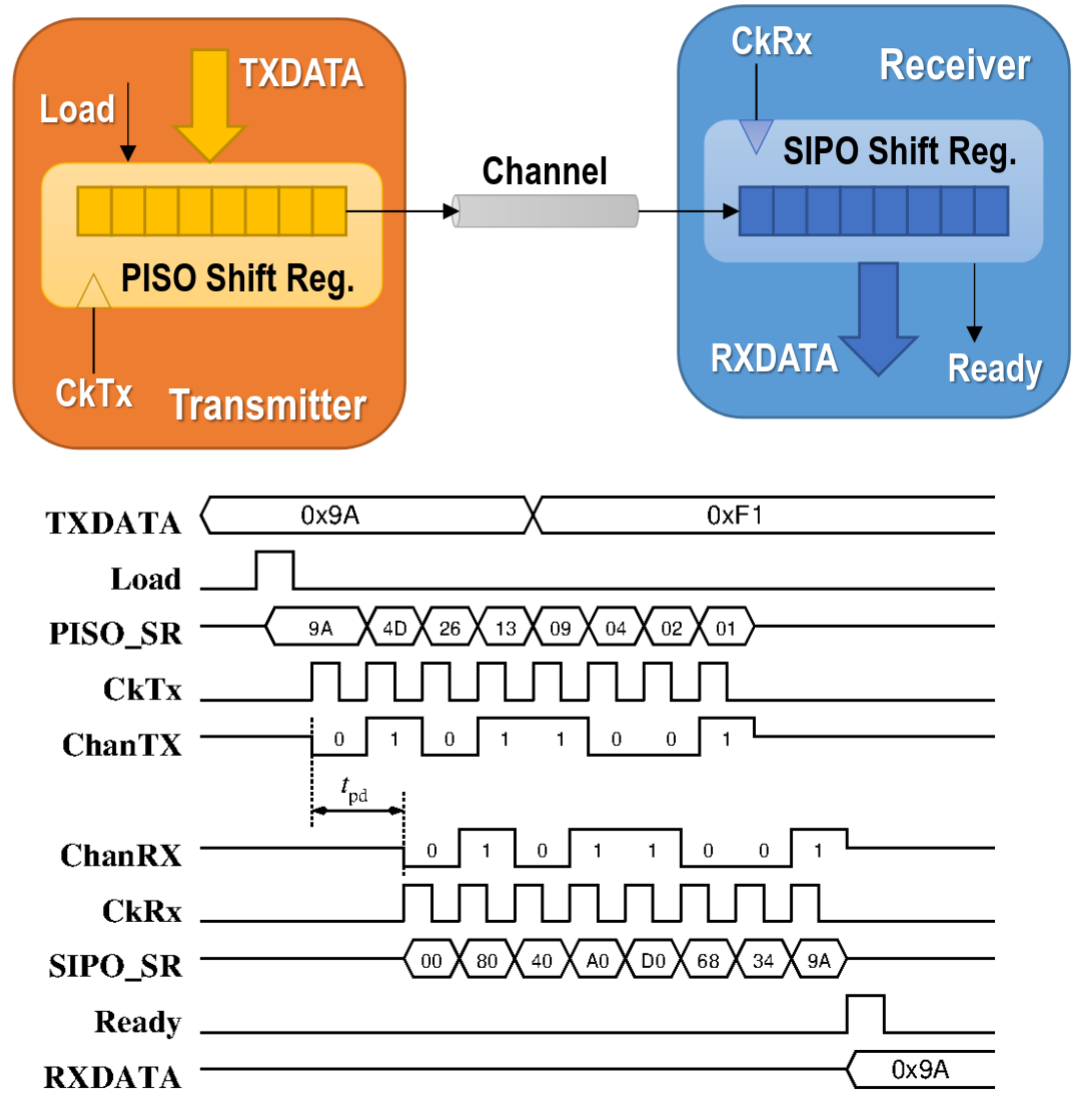
\includegraphics[scale=0.22]{../figures/serial_trans.png}
\end{center}

\par\smallskip

To enable full duplex transmission we may be tempted to have a transmitter and a receiver on each side, but we can get away with connecting the shift registers in a loop, such as:

\begin{center}
	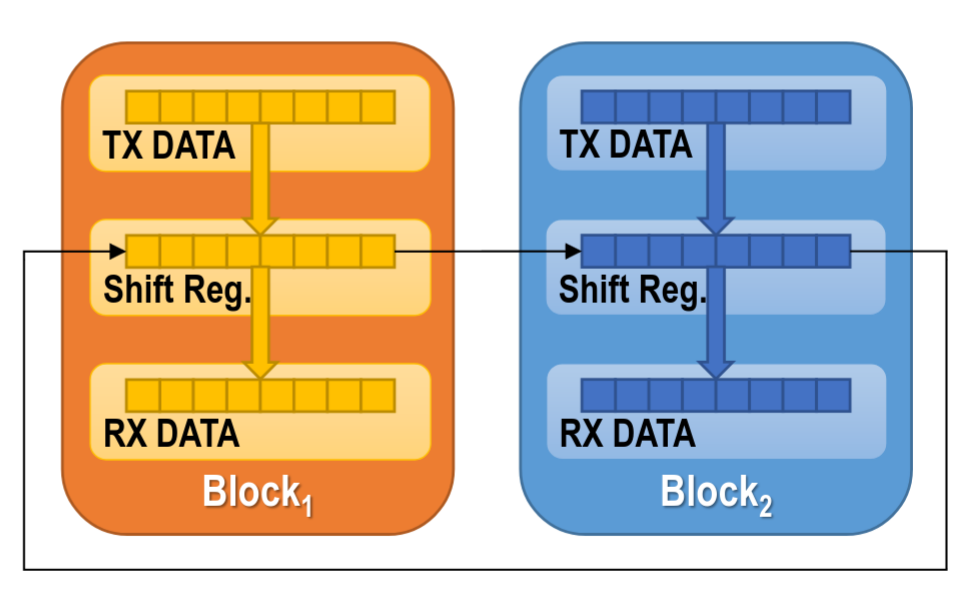
\includegraphics[scale=0.22]{../figures/serial_fduplex.png}
\end{center}

The pipeline each block (receiver/transmitter) follows is as follows:

\begin{enumerate}
	\item
	      Data to be transferred is in the TXDATA register of each block, respectively, and data from TXDATA is transferred to the Shift Register.
	      Blocks make this transfer without synchronizing.
	\item
	      Shift Registers of both blocks are clocked synchronously.
	      Data is shifted bit by bit from one shift register to the other.
	      After $n$ clock cycles (for $n$ bit shift registers), data has been transferred completely;
	\item
	      The contents of each Shift Register are transferred to the RXDATA register. Blocks make this last transfer without synchronizing.
\end{enumerate}

\subsubsection{Clock Sync.}

Proper clock transmission allows \textbf{bit} synchronization, which guarantees correct sampling of single bits (when loading in the receiver shift register). This needs to synchronzie the clock.
Higher protocol levels allow \textit{character} (endianess, ...) and \textit{message} synchronization message delimiters, ...).

The clock can be generated at the transmitter or receiver side, then sent to receiver or transmitter on a parallel line with respect to data. This is limited by skew, but at least (as we said) the skew is mostly the same between clock and data.

If sent by the receiver, the clock is also limited by transmission delay.

Clock can also be \textit{embedded} (\textit{Clock Data Recovery}, \textbf{CDR}): generated by transmitter, encoded in the data (presence of transitions), extracted by the receiver.
This means data changes periodically (define maximum interval between transitions), and continuously (to allow synchronization).

Lastly, we talk about \textit{isofrequential} clocks: in this case the transmitter and receiver have separate free running isofrequential clocks. Of course these need to be periodically synchronized.

\subsection{UART serial transmission}

Let's now talk about a real example of serial communications, which is \textbf{UART} (\textit{Universal Asynchronous Receiver Transmitter}).

UART consists of a point-to-Point serial communication, with:
\begin{itemize}
	\item Isofrequential independent clocks;
	\item Two serial wires;
	\item One for transmission from Block1 to Block2.
	\item One for transmission from Block2 to Block1.
\end{itemize}

Ground is of course included but not shown.

\begin{center}
	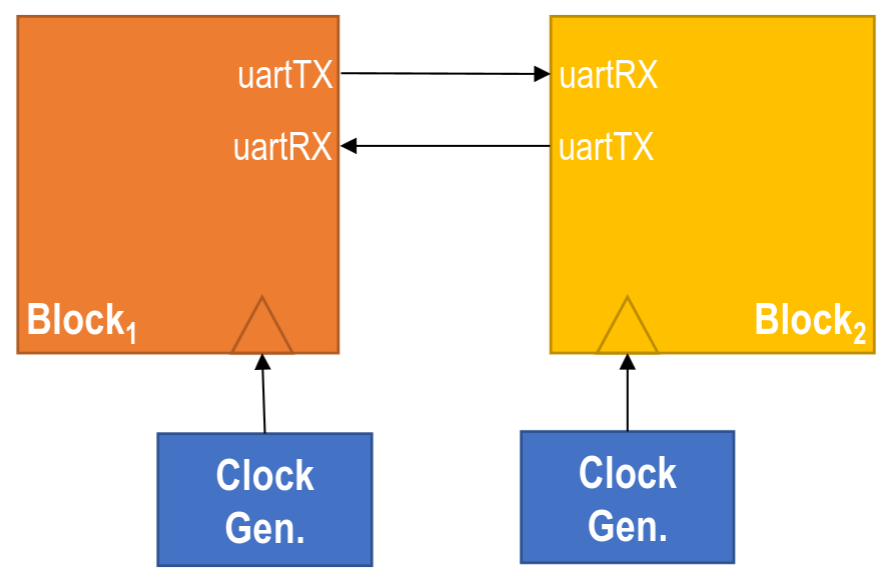
\includegraphics[scale=0.22]{../figures/uart.png}
\end{center}

As with most isofrequential systems, there's a periodic synchronization of the clocs.
After the synchronization the clocks run free.

\subsubsection{Character format}

Transmission in UART is character based.
Each transmitted bit lasts one clock cycle, and each transmission consists of a \textit{frame}, which contains a character of $n$ bits.

A frame has a defined format:
\begin{itemize}
	\item START BIT (1 bit);
	\item Character ($n$ bits, LSB first);
	\item PARITY BIT (1 bit, optional, might be absent);
	\item STOP BIT (1 or 2 bits).
\end{itemize}

Synchronization between clocks happens at the START BIT only.

\par\smallskip

We also need to talk about frame synchronization.

In the UART transmission format, an UART frame can start at any time.
Each bit nominally lasts one clock cycle, so:
$$
	t_\text{bit} = \frac{1}{f_\text{ck}}
$$

Character and parity bits are transmitted using standard NRZ encoding, so there are no guaranteed transitions.
How do we guarantee a transition in each frame (so that the receiver can notice when a transmission starts)?

The UART line is kept at logic 1 when idle, and STOP BITs are always at logic 1.
The START BIT is always a logic 0.
This means that either after an idle phase, or following the previous frame, the START BIT of a new frame always causes a 1 to 0 transition.

This START BIT transition allows synchronizing clocks at the beginning of a frame.
There is always at least a 0 to 1 transition (the first high data bit), as well, but its position is not known a priori, so it cannot be used for synchronization.

\subsubsection{Transmission parameters}

Transmitter and receiver should also agree on some parameters.

\begin{itemize}
	\item \textbf{Baud rate} (symbols per second): it is the nominal clock frequency $f_\text{ck}$ of the independent clocks. It corresponds to bps (bits per second) in this context, but symbols in general may represent more than one bit;
	\item \textbf{Number} $n$ of bits in a character;
	\item Presence and kind of \textbf{parity} bits (as we said the parity bit can be not present);
	\item Number of \textbf{stop} bits (either 1 of 2).
\end{itemize}

Note that the configuration of these parameters is outside of the UART protocol.

\subsubsection{Overhead}

We saw that UART transmits some bits (START, STOP, eventual parity...) which are not directty useful by themselves. These are \textbf{overheads}. The minimum overhead is given by the STOP - START transmission on frame start, so 2 bits.

We have that the maximum transmission rate depends on both:
\begin{itemize}
	\item \textbf{Baud Rate}:
	      The higher the baud rate, the higher the performance.
	      There are $f_\text{ck}$ bit times in a second;
	\item \textbf{Overhead}:
	      START BIT, Parity and STOP BITs do not carry information.
	      AS we said, the minimum overhead is 2 bits (START BIT, 1 STOP BIT).
	      The maximum overhead, on the other hand, is 4 bits (START BIT, Parity, 2 STOP BITs.
\end{itemize}

The equation for the ffective useful bit rate is:
$$
	\text{bit rate} = \frac{n}{n + o_h} f_\text{ck}
$$

Increasing $f_\text{ck}$ and $n$ might increase performance, but there are limits:
sampling is performed within a certain window where data is stable.

The window is between two active clock edges, where data potentially changes.
The window is defined by a set of parameters:
\begin{itemize}
	\item Voltage levels ($V_{OL}$, $V_{IL}$, $V_{OH}$, $V_{IH}$);
	\item Noise ($NML$, $NMH$);
	\item Timing (setup $t_{su}$, hold $t_h$, rising $t_r$ and falling $t_f$, slew rate, bandwidth).
\end{itemize}
Increasing the clock frequency makes the window smaller.
In addition to this clock drifting moves the sampling point outside the window after a certain number of bits without synchronization.
Once windows parameters are set, maximum $n$ and $f_\text{ck}$ can be computed

\subsubsection{UART performance}

Let's talk UART Performance.

For \textbf{long interconnections}, performance is limited by attenuation, distortion, noise.
These affect the vertical axis in the \textit{eye diagram} (see later).

Performance is also limited by unpredictable delays
These affect the horizontal axis in the eye diagram (see later).
It is improved by large voltage swings.

For \textbf{short interconnections}, erformance is limited by clock jitter and tolerances.
These affect the horizontal axis in the eye diagram (see later).

Note that interconnection length and speed are conflicting parameters: we can have a short and fast link, or a long and slow link.

\subsection{Eye diagrams}

An \textbf{eye diagram} defines the sampling window via signal waveforms at the receiver.
It is built considering all possible transitions between transmitted bits, and showing all transitions superimposed on the same graph.

Let's draw an eye diagram ourselves.
Let's start with a time interval equal to $t_\text{bit}$ and a voltage range between $V_{OL}$ and $V_{OH}$ for the given technology, out of the typical $0$ to $V_{cc}$ range.
Let's now assume for simplicity that $t_\text{rise} = t_\text{fall}$.

We start with ramps at the left side which start at $\frac{V_{OL} + V_{OH}}{2}$ and go toward $V_{OL}$ and $V_{OH}$ respectively, in time $t_\text{rise}$ (the down ramps at the rights side will be mirrors of this if $t_\text{fall} = t_\text{rise}$).
For large signals, we can use the \textbf{slew rate} $S_R$:
$$
	t_\text{rise} = \frac{V_{OH} - V_{OL}}{S_R}
$$

We then do the same thing on the right side, ensuring the total time away from $\frac{V_{OL} + V_{OH}}{2}$ is $t_\text{bit}$.

The result is shown below.

\begin{center}
	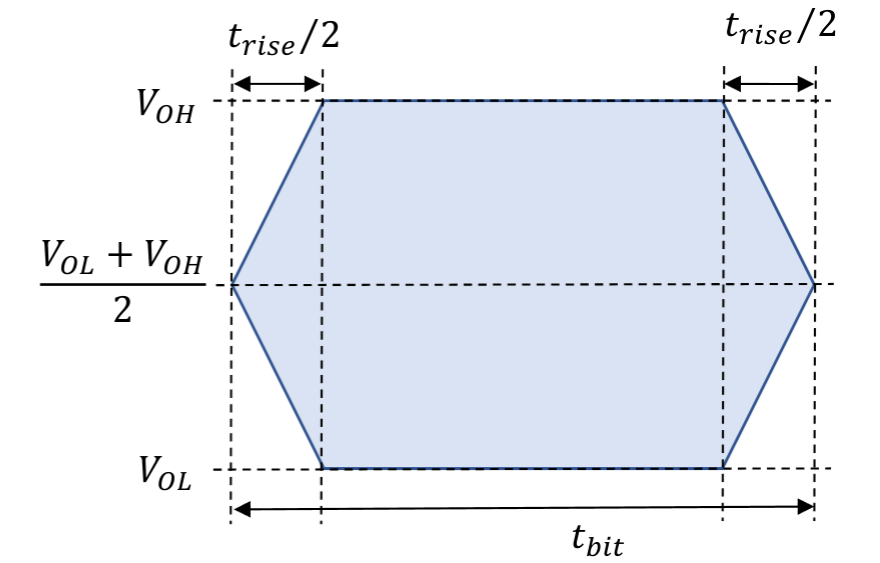
\includegraphics[scale=0.32]{../figures/eye_diag.png}
\end{center}

Let's note the noise margins in the graph and see where, in both sides (up and down) the signal is considered stable.
\begin{itemize}
	\item
	      We identify the value as high for a time $t_\text{stable}$ if the graph is above $V_{IH} + NM$.
	\item
	      We identify the value as low for a time $t_\text{stable}$ if the graph is below $v_{IL} - NM$.
\end{itemize}

\begin{center}
	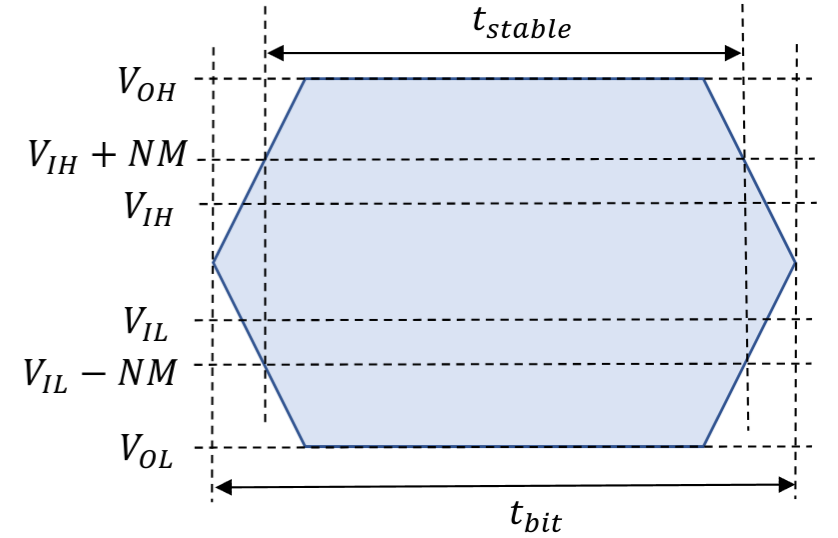
\includegraphics[scale=0.32]{../figures/eye_diag_nm.png}
\end{center}

This is still not enough, as the value has to be stable for enough time for the register to setup ($t_su$) and to hold ($t_h$).
This gives us the actual sampling window $t_w$, where we always have:
$$
	t_w < t_\text{stable} < t_\text{bit}
$$

Sampling inside the sampling window $t_w$ is always correct as:
\begin{itemize}
	\item The signal is stable;
	\item The signal has proper voltage levels;
	\item Setup and hold time are satisfied.
\end{itemize}

\begin{center}
	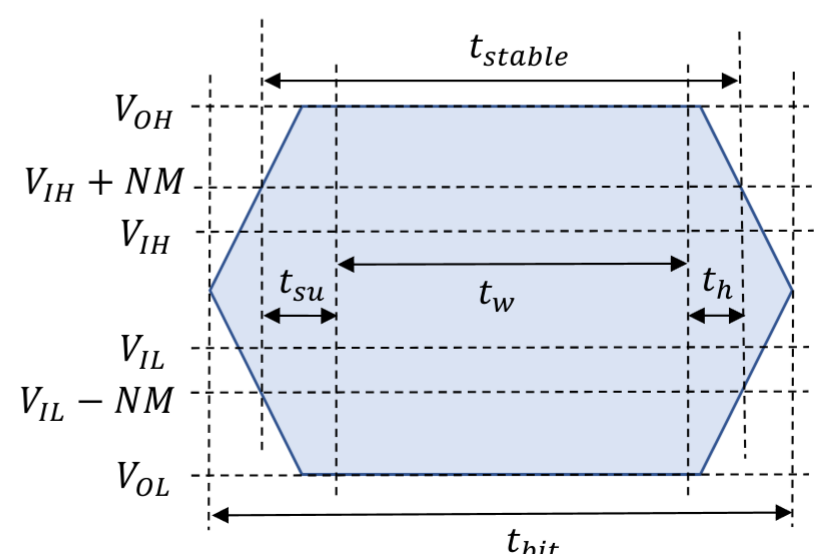
\includegraphics[scale=0.32]{../figures/eye_diag_su.png}
\end{center}

\par\smallskip

Now, immediately after synchronization, the receiver determines the best sampling instant.
We assume it is at the center of the sampling window.
The main isse is that clock drift eventually might get the sampling instant outside the sampling window.

This means we have 2 limitations:
\begin{itemize}
	\item \textit{Increasing $f_\text{ck}$ decreases the $t_w$ window, making the clock drift out faster.}

	      With perfect isofrequential clocks, we synchronize clocks on START BIT and always assume sampling happens within the sampling window for all successive bits.
	      So there is no limit to the number $n$ of consecutive bits, but here is still a limit to the maximum clock frequency.

	      With real rising and falling edge, we compute the window $t_w$ as:
	      \begin{center}
		      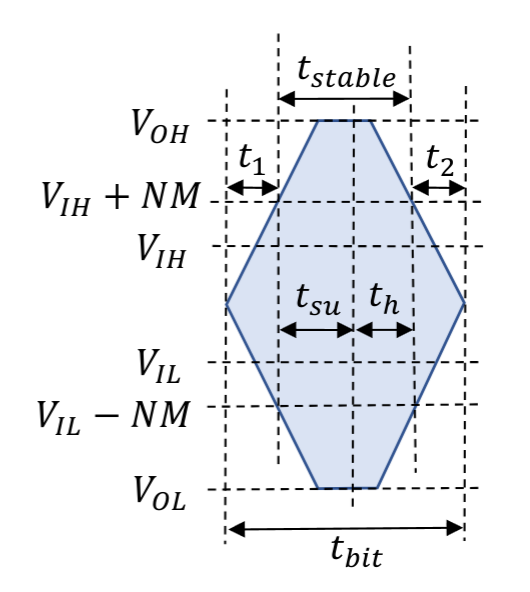
\includegraphics[scale=0.32]{../figures/clk_to_win.png}
	      \end{center}
	      $$
		      \begin{aligned}
			      t_1         & = \left( \frac{V_{IH} + NM}{V_{OH} - V_{OL}} - \frac{1}{2} \frac{V_{OH} + V_{OL}}{V_{OH} - V_{OL}} \right) t_\text{rise}, \quad t_2 = t_1 \\
			      f_\text{ck} & = \frac{1}{t_{su} + t_h + t_1 + t_2} = \frac{1}{t_{su} + t_h + 2 t_1}
		      \end{aligned}
	      $$

	      The maximum clock frequency limits the maximum performance.

	\item \textit{Increasing $n$ makes the clock to drift out towards the end of the transmission.}

	      Let's assume nominally isofrequential clocks with tolerances.
	      This means there's a relative error $\varepsilon$ (in percentage) from the nominal clock frequency at the receiver:
	      $$
		      \begin{cases}
			      f_\text{ck}  & = f_\text{nominal} \pm \delta_f   \\
			      t_\text{bit} & = t_\text{nominal} \pm \delta_t \
		      \end{cases}
		      \
		      \rightarrow
		      \
		      \begin{cases}
			      f_\text{ck}  & = f_\text{nominal} \pm \varepsilon_f \% \\
			      t_\text{bit} & = t_\text{nominal} \pm \varepsilon_t \%
		      \end{cases}
	      $$

	      With relative errors:
	      $$
		      \varepsilon_f = \frac{\delta_f}{f_\text{nominal}}, \quad
		      \varepsilon_t = \frac{\delta_t}{t_\text{nominal}}
	      $$

	      Because of this relative error, the sampling point from one bit to another differs by an amount:
	      $$
		      \Delta t = t_\text{bit}^{RX} - t_\text{bit}^{TX}
	      $$

	      In the worst case:
	      $$
		      \Delta t = t_\text{nominal} \cdot 2 \varepsilon
	      $$
	      Considering equal tolerances at transmitter and receiver, but in opposite directions.

	      As we were saying, drift may cause sampling outside the sampling window after a certain number of consecutive bits without re-synchronization.

\end{itemize}

\par\smallskip

In the eye diagram there is one degree of freedom: once we determine (estimate or measure) all parameters, we keep the clock frequency $f_\text{ck}$ and the number $n$ of consecutive bits unknown.
Fixed the clock frequency and its tolerance, we compute the maximum number of consecutive bits: $t_\text{bit}$ is known and equal to $t_\text{nominal}$ when drawing the eye diagram.

We can also do the reverse: fix the number of consecutive bits and the clock tolerance, compute the maximum clock frequency.
This leaves $t_\text{bit}$ as an unknown when drawing the eye diagram.

\end{document}
